\documentclass[font=default]{mpltx}
\usepackage{bm, ctex, array}
\usepackage{subfigure}
\usepackage{multirow}
% 以下至 \begin{document} 都仅是本文件为了方便额外定义的命令, 写报告时不需要.
\hypersetup{colorlinks=false}% 超链接带颜色
\usepackage{xcolor}
% 以上是本文件为了方便额外定义的命令, 写报告时不需要.
\linespread{1.5}
\begin{document}

\title{用传输式谐振腔观测铁磁共振} % 切合报告内容, 简短明确, 可以不同于讲义
\author{MaskedName} % 这里 \emailphone 一定要紧跟在 \author 后方
\emailphone{MyMail@stu.pku.edu.cn}{Tel}
% 如果改用 \email 则仅需要邮箱参数
\affiliation{北京大学物理学院\quad 学号: StudentID}
\date{\zhdate{2024/9/12}}
\begin{abstract}
铁磁体在受到相互垂直的恒定外磁场和射频交变磁场作用时,内部磁矩会发生共振现象,即铁磁共振(Ferromagnetic Resonance)。本实验以反射式速调管振荡器和传输式谐振腔为核心设备,深入研究了铁磁共振现象。实验中,首先观测了速调管振荡器的振荡模式,并测量了其中心频率和电子调谐范围。接着,通过测量传输式谐振腔的谐振曲线,计算了其有载品质因数。随后,采用简便方法并逐点测绘了输出功率与磁场的关系曲线,测量了铁磁共振的共振磁场和线宽,并计算了回磁比、郎德因子和弛豫时间。实验结果表明,传输式谐振腔在铁磁共振测量中具有较高的信号质量和较小的实验误差,验证了其作为铁磁材料磁动力学研究的有效工具。
\end{abstract}
\keywords{}

\maketitle

\section{引言}
铁磁共振(Ferromagnetic Resonance, FMR)是铁磁体在受到相互垂直的恒定外磁场和射频交变磁场作用时,内部磁矩发生的共振现象。磁矩在静磁场的作用下会绕着静磁场方向做拉莫尔进动,当外加交变磁场的频率与这种进动的自然频率相同时,会发生共振,导致能量的强烈吸收。通过铁磁共振可以测量铁磁体的磁矩、磁化率等物理量,也可以用于研究铁磁体的磁动力学性质。

本实验使用反射式速调管产生微波,并且用传输式谐振腔观测铁磁共振。反射式振荡器是一种真空电子器件,能够在微波频段内产生连续波信号。反射式速调管振荡器通过稳压电源为速调管提供较高的工作电压,以维持其内部电子的运动和微波信号的生成。由于其工作机制的要求,该振荡器在使用过程中能量消耗较大,相对于固态振荡源而言,其功耗较高。然而,反射式速调管振荡器在频率稳定性和相位噪声性能方面显著优于固态振荡器。传输式谐振腔是一种特殊的谐振腔,它的特点是在谐振腔内部有一个样品,样品的磁化会影响谐振腔的谐振频率。相较于传统的反射式谐振腔,传输式谐振腔在铁磁共振实验中具有更高的信号质量和较小的实验误差,因而在近年来得到了越来越多的应用。本实验通过测量传输式谐振腔的透射谱,可以得到铁磁共振的频率和线宽,从而得到回磁比、郎德因子以及弛豫时间等物理量。

\section{理论}
\subsection{传输式谐振腔}
在一个金属谐振腔两端加上矩形波导管,并在其两端加上带有耦合孔的金属板,就可以构成一个传输式谐振腔(见\autoref{fig:transmission_reso})。谐振腔的谐振频率与谐振腔的尺寸和形状有关,谐振腔发生谐振时,腔长$l$必须是半个波导波长的整数倍,也就是$$l=p\frac{\lambda_g}{2},\quad \lambda_g=\frac{\lambda}{\sqrt{1-\left(\frac{\lambda}{2a}\right)^2}}.$$这里$\lambda=c/f$为腔谐振频率对应的波长。微波进入谐振腔体中,部分能量被吸收,部分能量通过耦合孔透射到另一端,这样就形成了谐振腔的透射谱。谐振腔的透射谱是一个典型的洛伦兹线型,其品质因数$Q$是一个衡量谐振腔性能的重要参数,$Q$越大,谐振腔的透射谱越尖锐。有载品质因数$Q_L$由下式确定:$$Q_L=\frac{f_0}{|f_1-f_2|}.$$其中$f_0$为谐振腔的谐振频率,$|f_1-f_2|$为谐振腔的线宽(见\autoref{fig:reso_curve})。在实验中,我们可以通过测量谐振腔的透射谱,得到谐振频率和线宽,从而得到谐振腔有载品质因数$Q_L$。
\begin{figure}[h]
  \centering
  \begin{minipage}[t]{0.2\textwidth}
    \centering
    \vspace{-3cm}
    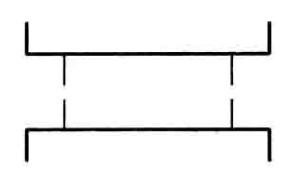
\includegraphics[width=\textwidth]{fig/transmission_reso.png}
    \caption{传输式谐振腔}
    \label{fig:transmission_reso} 
  \end{minipage}
  \hspace{1cm}
  \begin{minipage}[t]{0.35\textwidth}
    \centering
    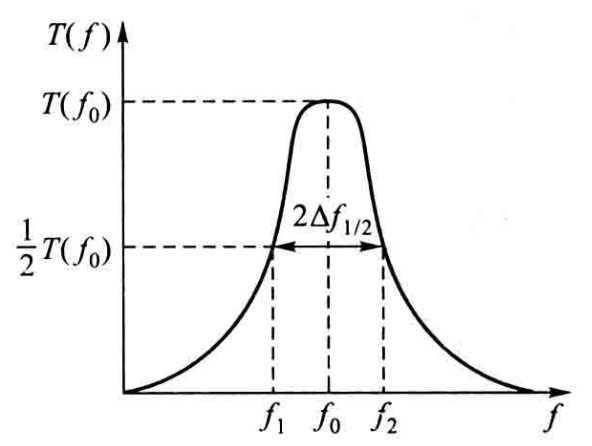
\includegraphics[width=\textwidth]{fig/reso_curve.png}
    \caption{传输式谐振腔的透射谱}
    \label{fig:reso_curve}
  \end{minipage}
\end{figure}

\subsection{反射式速调管的工作特性}
本实验中我们使用反射式速调管振荡器产生微波信号,其通过电子在电场中的加减速运动,利用电子的周期调制产生微波振荡。反射式速调管主要由阴极、谐振腔和反射极三部分构成(见\autoref{fig:reflex_klystron})。当阴极发射的电子进入谐振腔时,电子在谐振腔中受到电场的作用产生加速运动,穿过栅网,在反射极处受到反射极的电场作用,返回栅网。如此反复,当满足一定的条件时,电子在谐振腔中的运动会产生微波信号。

调节反射式速调管的振荡频率一般有两种方法:”电子调谐“和”机械调谐“。本实验中我们主要通过改变反射极电压从而实现调节振荡频率,即”电子调谐“。一个振荡模式半功率点对应的频率宽度称为”电子调谐范围“(\autoref{fig:elec_tuning} 中的$|f_1-f_2|$),半功率点对应的频宽与电压宽度的比值称为”平均电子调谐率“(\autoref{fig:elec_tuning} 中的$|(f_1-f_2)/(V_1-V_2)|$)。
\begin{figure}[h]
  \centering
  \begin{minipage}[t]{0.3\textwidth}
    \centering
    \vspace{-6cm}
    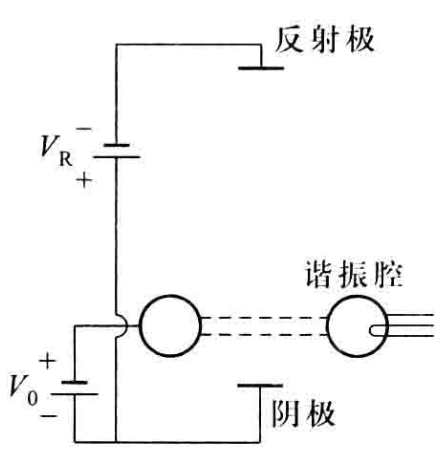
\includegraphics[width=\textwidth]{fig/reflex_klystron.png}
    \caption{反射式速调管原理图}
    \label{fig:reflex_klystron} 
  \end{minipage}
  \hspace{1cm}
  \begin{minipage}[t]{0.33\textwidth}
    \centering
    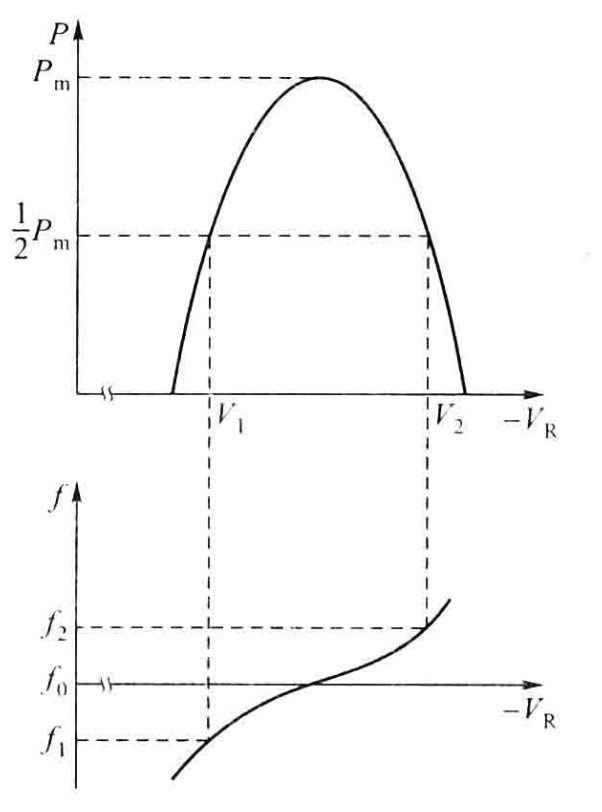
\includegraphics[width=\textwidth]{fig/elec_tuning.png}
    \caption{反射式速调管的电子调谐范围}
    \label{fig:elec_tuning}
  \end{minipage}
\end{figure}

\subsection{铁磁共振}
铁磁体的磁化系数很大,因此只需要外加比较小的磁场就可以使得铁磁体达到饱和磁化。铁磁体材料在外加恒定磁场$\bm{H}$的作用下,铁磁体的磁矩$\bm{M}$将从原来的平衡方向与$\bm{H}$夹角为$\theta$处开始沿着$\bm{H}$方向以角频率$\omega=\gamma H$进动,其中回磁比为$$\gamma=g\frac{\mu_0e}{2m}.$$式中$g$为郎德因子,$e$和$m$分别为电子的电荷量和质量。若只有恒定外磁场,由于铁磁体中存在阻尼作用,$\bm{M}$的振幅会不断衰减,以至于最后指向$z$方向。当再加入一个外加交变磁场,且外加磁场的频率(微波频率$\omega_r$)与进动的自然频率相同时,交变磁场被磁矩进动吸收的部分恰好可以抵消进动阻尼的能量损耗,即发生铁磁共振。此时,铁磁体的磁导率张量可以表示为
$$
\bm{mu}=\begin{pmatrix}
  \mu & -i\kappa & 0\\
  i\kappa & \mu & 0\\
  0 & 0 & \mu_{z}
\end{pmatrix},\quad (\mu=\mu'-i\mu'',\kappa=\kappa'-i\kappa'',\mu_z=\mu_z'-i\mu_z'').
$$
当发生共振的时候($\omega_r=\gamma H_r$),磁导率张量对角元虚部$\mu''$为最大值$\mu_r''$,所对应的磁场为共振磁场$H_r$。$\mu''=\mu_r''/2$所对应的磁场间隔$\Delta H=|H_1-H_2|$为铁磁共振的线宽(见\autoref{fig:ferro_reso})。

当磁场改变的时候,磁矩$\bm{M}$趋向平衡态的过程称为弛豫过程,弛豫过程的时间常数称为弛豫时间。铁磁共振的线宽$\Delta H$与弛豫时间$\tau$之间有关系:$$\tau=\frac{2}{\gamma\Delta H}.$$因此,通过测量铁磁共振的线宽,我们可以得到铁磁体的弛豫时间。
\begin{figure}
  \centering
  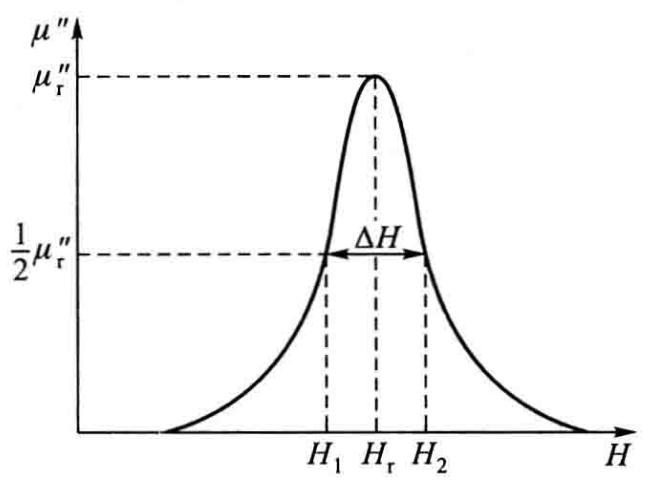
\includegraphics[width=0.35\textwidth]{fig/ferro_reso.png}
  \caption{铁磁共振曲线}
  \label{fig:ferro_reso}
\end{figure}

\subsection{用传输式谐振腔测量铁磁共振线宽}
当把铁磁体小样品放入谐振腔中时,会引起谐振腔谐振频率和品质因数的变化。如果将小样品看作一个微扰,同时将样品放在谐振腔内适当位置上,使得样品的磁效应和电效应分离,将小样品放在腔内微波磁场最大、电场为零的位置,则在$\rm TE_{10p}$矩形谐振腔中我们有
$$
\frac{f-f_0}{f_0}=-A(\mu'-1),\quad \Delta\left(\frac{1}{Q_L}\right)=2A\mu''.
$$其中$A$是与谐振腔的振荡模式、体积以及样品体积有关的常量$$A=\frac{2}{1+\left(\frac{l}{ap}\right)^2}\frac{V_S}{V_0}.$$其中$V_S$是样品体积,$V_0$是谐振腔体积。

要测量铁磁共振线宽,就要测量$\mu''$,即测量腔的有载品质因数$Q_L$,而$Q_L$的变化可以通过腔的输出功率变化来测量。若铁氧体小球放在腔内微波磁场最大处,则在谐振腔始终调谐时有
$$
T(f_0)=\frac{P_{\text{out}}(f_0)}{P_{\text{in}}(f_0)}=\frac{4Q^2_L}{Q_{e1}Q_{e2}}\Longrightarrow P_{\text{out}}(f_0)=\frac{4P_{\text{in}}(f_0)}{Q_{e1}Q_{e2}}Q^2_L\propto Q^2_L.
$$其中$Q_{e1}$和$Q_{e2}$分别是输入端和输出端的品质因数。因此,通过测量输出功率的变化,我们可以得到铁磁共振的线宽。

可以推导出,半功率点$P_{\frac12}$(即$\mu''=\mu_r''/2$的点)的表达式为$$P_{\frac12}=\frac{4P_0}{(\sqrt{P_0/P_r}+1)^2}.$$其中$P_0$为远离铁磁共振区域时谐振腔的输出功率,$P_r$为共振时的输出功率(见\autoref{fig:P-H_relation})。值得注意的是,因为测量过程中,样品的$\mu'$会使得谐振腔的谐振频率发生偏移(频散效应),因此我们需要考虑对频散效应进行修正,通过一系列推导,我们可以得到半共振点对应的功率应为
$$
P_{\frac12}=\frac{2P_0P_r}{P_0+P_r}.
$$

\begin{figure}
  \centering
  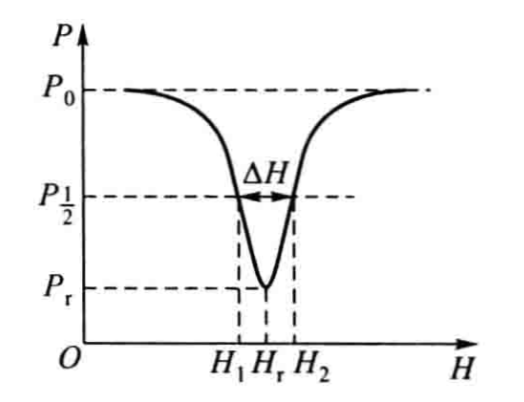
\includegraphics[width=0.35\textwidth]{fig/P-H_relation.png}
  \caption{输出功率和磁场的关系曲线}
  \label{fig:P-H_relation}
\end{figure}

\section{实验内容}
本实验的装置示意图如\autoref{fig:ex_setup} 所示,这是一套在3 cm 波段上进行观测的实验装置,可以同时做观测传输式腔的工作特性和铁磁共振两个方面的实验。本实验中我们通过晶体检波接头接入检流计的方式测量微波功率。
\begin{figure}
  \centering
  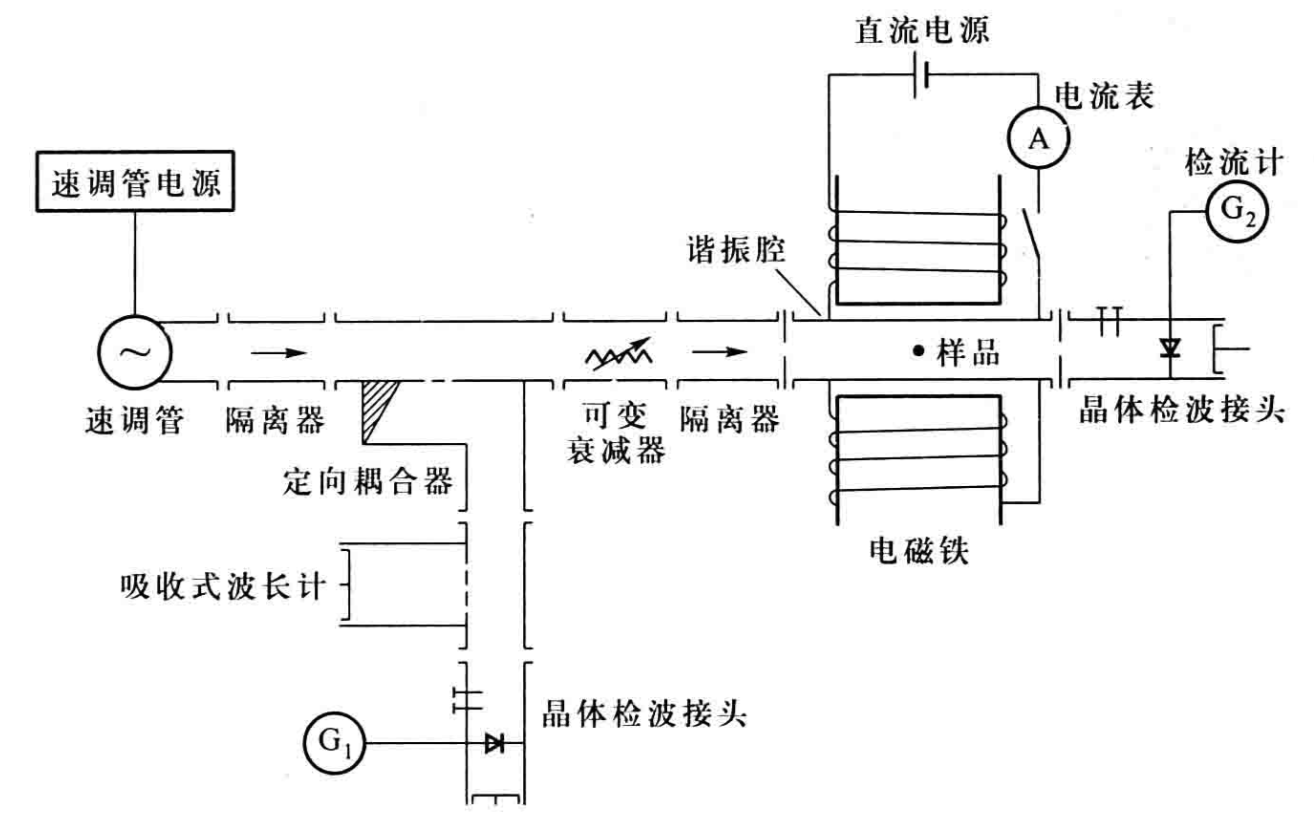
\includegraphics[width=0.7\textwidth]{fig/ex_setup.png}
  \caption{观测铁磁共振的实验装置}
  \label{fig:ex_setup}
\end{figure}
\subsection{观察速调管的振荡模,测量一个振荡模中心频率和电子调谐范围}
打开信号发生器的电源,预热30分钟。将断-连续-调制旋钮置于合适位置,并且将速调管的衰减旋钮置于衰减量最小处。调节反射极旋钮,电流示数从开始增大要结束减小为一个振荡模,记下最大电流刻度,并且调谐得到该振荡模的中心频率。之后再分别顺/逆时针调节反射极旋钮,在电流读数为最大读数的一半时,用同样的方法调谐,记录对应的频率。通过这两个频率的差值,我们可以得到电子调谐范围。
\subsection{测量传输式腔的谐振曲线,测量腔的有载品质因数}
打开检流计。在信号发生器的电流最大位置附近慢慢调节反射极旋钮,检流计的读数非均匀的由小变大再变小,这就是谐振曲线。检流计读数最大时,就是谐振腔达到谐振的位置,调整波长表旋钮记录对应的频率。再分别顺/逆时针调节反射极旋钮,在检流计读数为最大读数的一半时,用同样的方法调谐,记录对应的频率。通过这两个频率的差值,我们可以得到谐振腔的线宽。之后,我们可以通过公式$$Q_L=\frac{f_0}{|f_1-f_2|},$$得到谐振腔的有载品质因数。

\subsection{测量铁磁共振的磁场和线宽,并逐点测绘输出功率和磁场的曲线}

打开励磁直流电源,并且改变滑动变阻器的阻值,记录检流计$\rm G_2$的最大最小读数、中点读数、以及它们所对应的电流表的读数。反复测量3次,每次测量时都要重新对谐振腔调谐。最后利用电流表读数查表得到磁场的值,确定共振磁场和线宽。

随后测绘输出功率和磁场的关系曲线。将变阻器阻值调至合适位置,改变变阻器的阻值,逐点测量检流计读数以及对应的电流表读数,记录下来,测量20到40个点。然后查表得到电流对应的磁场的值,绘制输出功率和磁场的关系曲线。

\section{实验结果与分析}
\subsection{观测速调管的振荡模和传输式腔的谐振曲线}
\subsubsection{测量一个振荡模的中心频率的电子调谐范围}
调节波长表使得电流表示数最小,此时对应的波长即为谐振频率对应的波长。顺/逆时针调节反射极使得电流表示数为最大值的一半,此时对应的波长即为半功率点对应的波长。实验中测量结果如\autoref{tab:elec_reso} 所示。
\begin{table}[h]
  \label{tab:elec_reso}
  \caption{电子调谐中心波长和调谐范围测量结果}
  \vspace{0.2cm}
  \begin{tabular}{c|c|c|c}
    \hline
  反射极调节           & 电流表$\rm G_1$示数($\mu$A) & 波长表   & 对应频率(MHz)\footnote{这里的对应频率是由实验室提供的波长计刻度曲线表算出来的,表中给出的$f$和$\lambda$的拟合关系为:$f=a+b\lambda=10014.79-211.27\lambda\ (MHz)$。注意我们记录波长表的时候只记录了四位有效数字,但是在对应频率的计算结果中我们保留了五位有效数字。这是因为从上面的$f$和$\lambda$关系中我们可以知道0.005的波长变化就会影响1MHz的对应频率,因此在计算频率的时候,应该要算到小数点后一位。} \\\hline\hline
  使得电流示数最大        & 53.0  & 3.800 & 9212.0 \\\hline
  顺时针使得电流示数为最大的一半 & 26.5  & 3.679 & 9237.5 \\\hline
  逆时针使得电流示数为最大的一半 & 26.5  & 3.942 & 9182.0 \\\hline
  \end{tabular}
\end{table}

因此我们可以得到电子调谐中心频率为$$f_0=9212.0\ \rm MHz,$$电子调谐范围为$$|f_1-f_2|=55.5\ \rm MHz.$$

\subsubsection{测量腔的有载品质因数}
在信号发生器电流达到最大值的附近,缓慢调节反射极旋钮,检流计的读数会从小逐渐增大到峰值后再逐渐减小,这个过程形成了谐振曲线。通过调节反射极,使检流计读数达到最大值,并记录此时波长表的读数。接着,顺时针或逆时针调节反射极,使检流计读数降至最大值的一半,记录此时的波长表数值。实验中测量结果如\autoref{tab:reso_curve2} 所示。
\begin{table}[h]
  \label{tab:reso_curve2}
  \caption{传输式腔的谐振曲线测量结果}
  \vspace{0.2cm}
  \begin{tabular}{c|c|c|c}
    \hline
  反射极调节           & 检流计$\rm G_2$的格数 & 波长表   & 对应频率(MHz)\footnote{这里我们计算对应频率的时候保留五位小数,具体计算方法见\autoref{tab:elec_reso} 的脚注。} \\\hline\hline
  使得电流示数最大        & 72.8  & 3.777 & 9216.8 \\\hline
  顺时针使得电流示数为最大的一半 & 36.4  & 3.770 & 9218.3 \\\hline
  逆时针使得电流示数为最大的一半 & 36.4  & 3.787 & 9214.7 \\\hline
  \end{tabular}
\end{table}

因此我们得到谐振腔的共振频率为$$f_0=9216.8\ \rm MHz.$$
传输式谐振腔的有载品质因数为$$Q_L=\frac{f_0}{|f_1-f_2|}=2560.$$
\subsection{观测铁磁共振}
\subsubsection{简便方法测量共振磁场和线宽}
首先将变阻器的阻值调到最大值,将直流电压调整到合适的位置。慢慢调小变阻器的阻值,可以观察到在很大的阻值范围内,检流计的示数几乎没有变化,但是在一个很小的范围内,检流计的读数会迅速的先变小再变大。测量3次之后得到的结果如\autoref{tab:ferro_reso} 所示。
\begin{table}[h]
  \caption{用简便方法测量共振磁场和线宽结果}
  \vspace{0.2cm}
  \label{tab:ferro_reso}
  \begin{tabular}{c|c|cc|cc|cc}
    \hline
     & $P_0$\footnote{检流计$G_2$的格数。在变阻器阻值很大的时候,调整变阻器的阻值几乎不会对检流计的示数造成太大的变化,因此这里的$P_0$就取变阻器阻值最大时对应的检流计示数。} & $P_r$ & $I_r(\text{A})$\footnote{这里是检流计示数最小的时候对应的电流表的示数,也就是\autoref{fig:P-H_relation} 中的$H_r$对应的励磁电流的大小。之后测量的$I_1$和$I_2$分别对应\autoref{fig:P-H_relation} 中的$H_1$和$H_2$点。}  & $P_{\frac12}$\footnote{这里的$P_{\frac12}$是根据频散效应修正后的公式$P_{\frac12}=2P_0P_r/(P_0+P_r)$得到。} & $I_1(\text{A})$  & $P_{\frac12}$ & $I_2(\text{A})$  \\\hline\hline
  1  & 90.2 & 37.4 & 2.262 & 52.9  & 2.167 & 52.9  & 2.347 \\\hline
  2  & 91.0 & 36.9 & 2.244 & 52.5  & 2.137 & 52.5  & 2.337 \\\hline
  3  & 91.0 & 37.0 & 2.261 & 52.6  & 2.147 & 52.6  & 2.349 \\\hline
  平均\footnote{在下面我们会看到磁场和电流是线性关系,所以求电流的平均值和求磁场的平均值得到的结果是一样的。为了计算简洁,我们这里只取电流的平均值,之后再计算对应磁场的平均值。} & /    & /    & 2.256 & / & 2.150  & /  &  2.344  \\\hline
  \end{tabular}
\end{table}

实验室中提供的电流-磁场对照表(2023.2.20测)给出电流和磁场的拟合的线性关系$$H=1390\times I\text{(A)}+140\ \text{(Oe)}.$$由\autoref{tab:ferro_reso} 中的数据我们可以计算得到
$$H_r=3275\ {\text{Oe}},\quad H_1=3129\ {\text{Oe}},\quad H_2=3399\ {\text{Oe}}.$$
因此我们得到共振磁场为$$H_r=3275\ {\text{Oe}},$$线宽为$$\Delta H=|H_2-H_1|=270\ {\text{Oe}}.$$

\subsubsection{逐点测绘输出功率和磁场的曲线,计算回磁比、郎德因子和弛豫时间}
再次调谐之后,从大到小改变变阻器的阻值,逐点测量检流计读数$P$和对应的电流表读数$I$,注意由于磁滞效应,变阻器阻值只能向一个方向变动。测量结果如\autoref{fig:ferro_reso_curve}所示(测量原始数据在\autoref{tab:ferro_reso_curve} 中)。
\begin{figure}
  \centering
  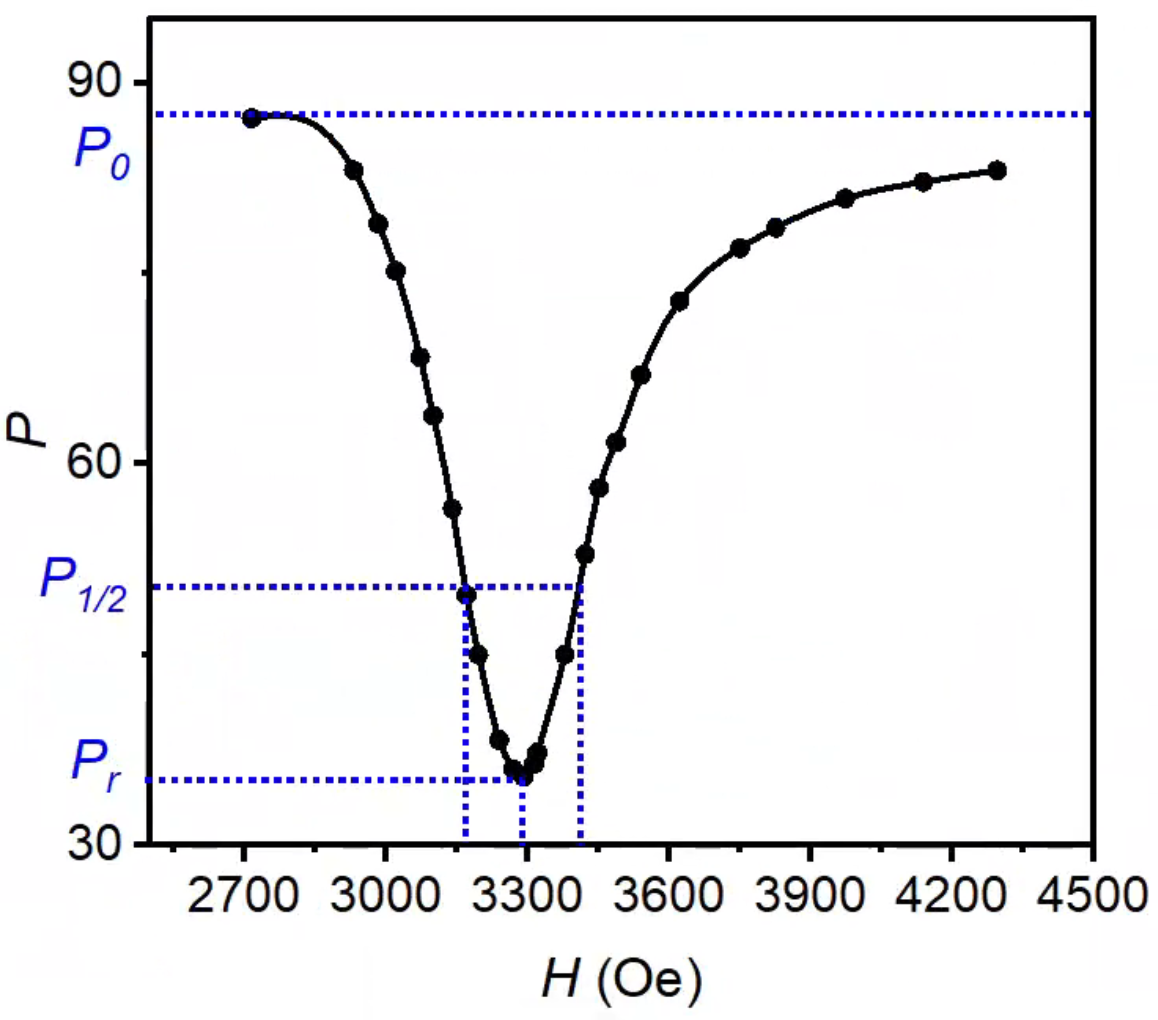
\includegraphics[width=0.55\textwidth]{fig/P-H_relation_exp.png}
  \caption{测量得到的$P-H$曲线}
  \label{fig:ferro_reso_curve}
\end{figure}

从\autoref{fig:ferro_reso_curve} 中我们可以看到,$P-H$曲线的形状和我们预期的一样,即在共振磁场附近,输出功率会有一个明显的下降。我们可以通过计算得到半功率点的输出功率$P_{\frac12}$和对应的磁场$H_1$和$H_2$。并且通过这些值来计算回磁比$\gamma$、郎德因子$g$和弛豫时间。

根据\autoref{tab:ferro_reso} 我们可以得到$H_0=3290\ \text{Oe}$,于是回磁比为($f_0$在“测量腔的有载品质因数”一节中已经测过,为9216.8 MHz)$$\gamma=\frac{2\pi f_0}{H_0}=1.760\times 10^{7}\ {\rm Oe^{-1}\cdot s^{-1}}=2.212\times10^{5}\ {\rm m\cdot A^{-1}\cdot s^{-1}}.$$
郎德因子为$$g=\frac{2m\gamma}{\mu_0e}=2.002.$$
从\autoref{fig:ferro_reso_curve} 我们读出线宽约为$$\Delta H=|H_2-H_1|=243\ \text{Oe}=1.93\times 10^{4}\ {\rm A\cdot m^{-1}},$$因此弛豫时间为$$\tau=\frac{2}{\gamma\Delta H}=4.68\times 10^{-10}\ \text{s}.$$

\section{结论}
本实验通过观测速调管的振荡模,成功测量了中心频率为9212.0 MHz的振荡模,电子调谐范围为55.5 MHz。传输式腔的谐振曲线测量结果显示,谐振频率为9216.8 MHz,有载品质因数为2560。
铁磁共振实验中,简便方法测得的共振磁场为3275 Oe,线宽为270 Oe。逐点测绘输出功率与磁场的关系曲线进一步验证了共振现象,并计算得到回磁比为$2.212\times10^5\ {\rm m\cdot A^-1\cdot s^-1}$,郎德因子为$g=2.002$,和我们已知的结果相对应。最后我们算出弛豫时间为$\tau =4.68\times10^{-10} \text{s}$,数量级在我们的预测范围之内。

实验结果证实了传输式谐振腔在铁磁共振测量中的有效性和准确性,为铁磁材料的磁动力学性质研究提供了可靠的实验数据和分析方法。

\begin{thebibliography}{}

  \bibitem{book} 吴思诚, 荀坤. 近代物理实验(第四版). 北京: 高等教育出版社, 2015.
\end{thebibliography}
\appendix

\section{逐点测绘输出功率和磁场的曲线的原始数据}
逐点测绘输出功率和磁场的曲线的原始数据如\autoref{tab:ferro_reso_curve} 所示。
\begin{table}[h]
  \caption{逐点测绘输出功率和磁场的曲线的原始数据}
  \label{tab:ferro_reso_curve}
  \vspace{0.2cm}
  \begin{tabular}{>{\centering\arraybackslash}p{2cm}|>{\centering\arraybackslash}p{2cm}|>{\centering\arraybackslash}p{2cm}}
    \hline
  $I$(A) &  $H$(Oe)  & $P$ \\\hline
  1.852 & 2714.28 & 87.2 \\
  2.008 & 2931.12 & 83.1 \\
  2.045 & 2982.55 & 78.9 \\
  2.072 & 3020.08 & 75.2 \\
  2.109 & 3071.51 & 68.4 \\
  2.129 & 3099.31 & 63.8 \\
  2.158 & 3139.62 & 56.5 \\
  2.18  & 3170.2  & 49.7 \\
  2.198 & 3195.22 & 45   \\
  2.23  & 3239.7  & 38.3 \\
  2.251 & 3268.89 & 36   \\
  2.267 & 3291.13 & 35.4 \\
  2.283 & 3313.37 & 36.4 \\
  2.288 & 3320.32 & 37.3 \\
  2.33  & 3378.7  & 45   \\
  2.361 & 3421.79 & 52.9 \\
  2.382 & 3450.98 & 58.1 \\
  2.408 & 3487.12 & 61.7 \\
  2.446 & 3539.94 & 67   \\
  2.505 & 3621.95 & 72.8 \\
  2.597 & 3749.83 & 77   \\
  2.652 & 3826.28 & 78.6 \\
  2.758 & 3973.62 & 80.9 \\
  2.877 & 4139.03 & 82.2 \\
  2.99  & 4296.1  & 83.1\\\hline
  \end{tabular}
\end{table}

\end{document}
